\section{O que mudou durante o treino}
\label{sec:treino}
Em cada minibatch, a rede produz dois logits por resenha e a entropia
cruzada mede a perda frente ao rótulo. O \textit{backward} calcula os
gradientes dos embeddings, filtros e saída. Limitamos sua norma global a
1 antes da atualização. Os embeddings começam com distribuição normal de
desvio 0,1 e linha de padding zero. Os filtros usam inicialização de He
e a saída, Xavier \cite{prince}.

\subsection{Como escolhemos a taxa e a época}
\begin{tabularx}{\linewidth}{@{}lXr@{}}
\toprule
\tabelahead{Otimizador} & \tabelahead{Taxas testadas} & \tabelahead{Escolhida}\\
\midrule
SGD & 0,001 \quad 0,03 \quad 0,3 & 0,3\\
SGD com momentum 0,9 & 0,001 \quad 0,01 \quad 0,1 & 0,1\\
Adam & 0,0003 \quad 0,001 \quad 0,003 & 0,001\\
\bottomrule
\end{tabularx}
\legendinha{Tabela 3. Três sementes por célula (17, 29 e 43), minibatches de
64 e orçamento de 12 épocas. A CNN base tem larguras 3/4/5, cem filtros por
largura e dropout de 0,5.}

Na mesma semente, fixamos pesos iniciais e ordem dos minibatches. Salvamos
a época de menor CE de validação de cada treino e escolhemos a taxa com a
menor média dessa perda entre sementes. A época zero é a inicialização.

\medskip
\noindent\makebox[\linewidth]{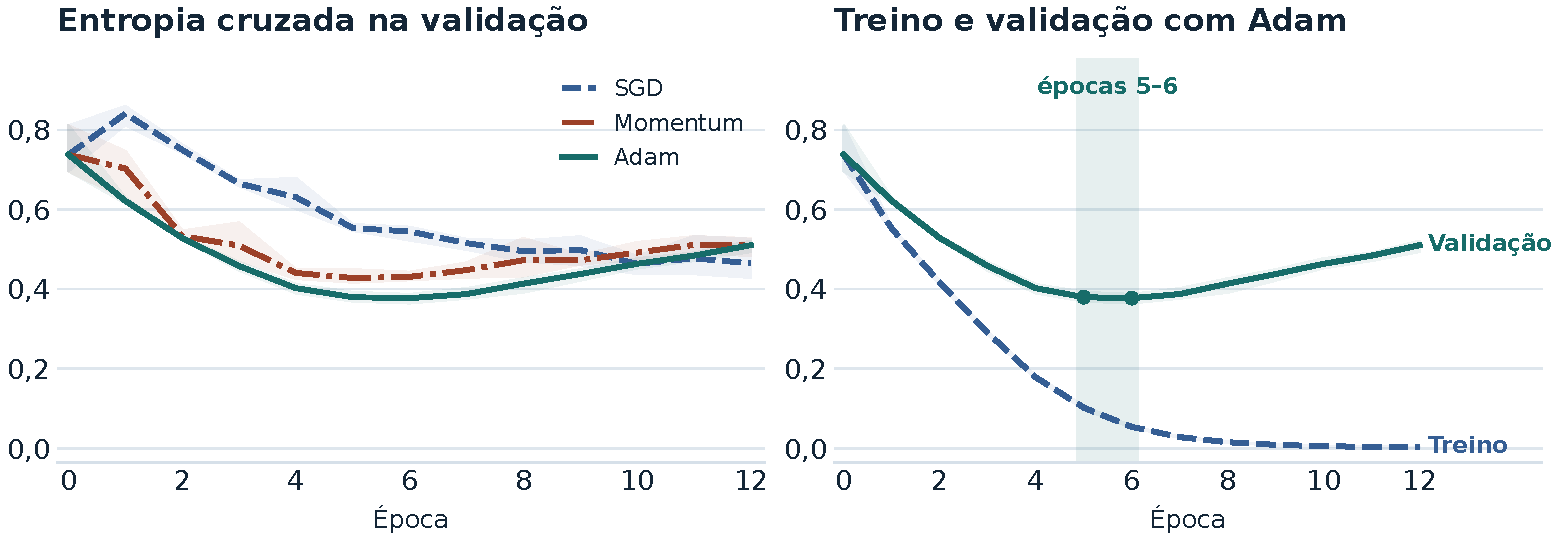
\includegraphics[width=.89\linewidth]{figuras/otimizacao.pdf}}
\legendinha{Figura 2. As linhas são médias e as faixas cobrem mínimo e máximo
entre sementes. À esquerda, cada otimizador usa sua taxa escolhida. À direita,
a perda de treino com Adam continua caindo depois da melhor região de
validação. Os checkpoints de Adam vêm das épocas 5 e 6.}

\subsection{Largura, número de filtros e dropout}
Fizemos 42 treinos de CNN. Além dos 27 acima, nove variaram largura ou
número de filtros e seis variaram dropout. Na auditoria sequencial,
larguras 3 e 5 isoladas (100 filtros) chegaram a 81,27\% e 80,94\% de
acurácia. A combinação 3/4/5 chegou a 81,95\% com 300 filtros e a
81,64\% com 96. Com dropout de 0,8, a acurácia foi 80,44\%. \fonte{results/sequences/summary.json}{Grade e métricas por semente}.
